% ------------------------------------------------------------
% Chi tiết hiện thực: mã nguồn, công nghệ, tham số (bổ sung Chương 3 kiến trúc)
% ------------------------------------------------------------
\subsection{Chi tiết hiện thực các thành phần}
\label{subsec:implementation_components}

Phần này bổ sung cho thiết kế kiến trúc ở Chương~\ref{sec:system_design}: ánh xạ thư mục/tệp,
luồng ETL, lược đồ vật lý trong SQLite, truy vấn OLAP tham chiếu, dashboard và mô hình khai phá.

\subsubsection{Ánh xạ tệp và công nghệ nền}

\begin{itemize}
  \item \textbf{Nguồn:} \texttt{data/flights.csv}, \texttt{data/airlines.csv}, \texttt{data/airports.csv}.
  \item \textbf{ETL:} thư mục \texttt{etl/} (\texttt{extract.py}, \texttt{transform.py}, \texttt{load.py}),
        điều phối bởi \texttt{pipeline.py}; ngôn ngữ Python 3.10+, thư viện \texttt{pandas}, \texttt{numpy}.
  \item \textbf{Kho:} SQLite \texttt{warehouse/airline\_dw.db}, DDL trong \texttt{warehouse/schema.sql}.
  \item \textbf{OLAP tham chiếu:} \texttt{queries/olap\_queries.sql} (9 nhóm truy vấn).
  \item \textbf{Dashboard:} Streamlit + Plotly, điểm vào \texttt{dashboard/app.py}, các trang trong \texttt{dashboard/}.
  \item \textbf{Khai phá:} thư mục \texttt{mining/} (huấn luyện, so sánh mô hình, artifact \texttt{.pkl}, báo cáo HTML).
\end{itemize}

% --- ETL ---
\subsubsection{Pipeline ETL}

Pipeline gồm 4 bước tuần tự trong \texttt{pipeline.py}:

\paragraph{Bước 1 --- Đọc và transform dimension nhỏ.}
\texttt{airlines.csv} và \texttt{airports.csv} đọc toàn bộ vào RAM; transform thành \texttt{dim\_airline}, \texttt{dim\_airport}
qua \texttt{transform.py}. \texttt{flights.csv} được quét một lần với chunk lớn (300.000 dòng) để thu thập ngày duy nhất,
rồi xây \texttt{dim\_date} bằng \texttt{pd.to\_datetime} vectorized.

\paragraph{Bước 2 --- Khởi tạo schema.}
Thực thi \texttt{warehouse/schema.sql} qua \texttt{conn.executescript()}. Tối ưu ghi SQLite:
\begin{lstlisting}[language=SQL, caption={SQLite PRAGMA tối ưu ghi}]
PRAGMA journal_mode = WAL;
PRAGMA synchronous = NORMAL;
\end{lstlisting}

\paragraph{Bước 3 --- Nạp dimension và lookup maps.}
Sau khi nạp các bảng chiều, pipeline truy vấn để xây dictionary ánh xạ surrogate key (khóa thay thế):
\texttt{airline\_map}, \texttt{airport\_map}, \texttt{date\_map}, \texttt{delay\_reason\_map};
dùng trong bước 4 với \texttt{pandas.Series.map()} (vectorized).

\paragraph{Bước 4 --- Streaming \texttt{fact\_flights}.}
Vòng lặp: đọc chunk $\rightarrow$ \texttt{transform\_chunk} $\rightarrow$ INSERT batch $\rightarrow$ giải phóng RAM.
\begin{lstlisting}[language=Python, caption={Vòng lặp streaming trong \texttt{pipeline.py}}]
CHUNK_SIZE   = 100_000   # row/chunk ~ 120 MB RAM
INSERT_BATCH = 50_000    # row/INSERT into SQLite

for chunk in stream_flights(chunksize=CHUNK_SIZE):
    fact = transform_chunk(chunk, airline_map, airport_map,
                           date_map, delay_reason_map)
    del chunk
    load_fact_flights(conn, fact, chunksize=INSERT_BATCH)
    del fact
\end{lstlisting}

\paragraph{Tối ưu kiểu dữ liệu (\texttt{extract.py}).}
Dùng \texttt{float32}/\texttt{int8}/\texttt{int16} thay mặc định \texttt{float64}/\texttt{int64} để giảm RAM mỗi chunk
(khoảng 120~MB thay vì $\approx$300~MB với chunk 100\,000 dòng).

\paragraph{Phân loại nguyên nhân trễ (vectorized).}
Dùng \texttt{numpy.select} thay \texttt{apply} theo dòng:
\begin{lstlisting}[language=Python, caption={\texttt{np.select} gán \texttt{delay\_reason\_key}}]
conditions = [
    df["WEATHER_DELAY"]       > 0,
    df["AIR_SYSTEM_DELAY"]    > 0,
    df["LATE_AIRCRAFT_DELAY"] > 0,
    df["AIRLINE_DELAY"]       > 0,
    df["SECURITY_DELAY"]      > 0,
]
df["delay_reason_key"] = np.select(
    conditions, choices, default=delay_reason_map["NO_DELAY"]
)
\end{lstlisting}

\paragraph{Chiến lược xử lý missing data:}
\begin{itemize}
  \item Các cột delay: \texttt{fillna(0.0)} (\texttt{NaN} $\equiv$ không có trễ loại đó).
  \item Bản ghi thiếu \texttt{AIRLINE}, \texttt{ORIGIN\_AIRPORT} hoặc \texttt{DESTINATION\_AIRPORT}: loại ở \texttt{extract.py}.
  \item Không map được FK chiều: \texttt{dropna(subset=[...])} trong \texttt{transform\_chunk}.
\end{itemize}

\noindent \textbf{Dữ liệu sau khi nạp vào kho:}

Pipeline ETL xử lý ba tệp CSV đầu vào và tạo ra Data Warehouse SQLite
với cấu trúc Star Schema đã thiết kế. Bảng~\ref{tab:etl_stats} tóm tắt
khối lượng dữ liệu trước và sau làm sạch.

\begin{table}[H]
\centering
\caption{Thống kê dữ liệu sau quá trình ETL}
\begin{tabular}{|l|r|r|r|}
\hline
\textbf{Bảng} & \textbf{Bản ghi thô} & \textbf{Bản ghi sau làm sạch} & \textbf{Tỷ lệ giữ lại} \\ \hline
\texttt{fact\_flights} & 5.819.079 & 5.332.914 & 91{,}65\% \\ \hline
\texttt{dim\_airline}  & 14        & 14             & 100\%  \\ \hline
\texttt{dim\_airport}  & 322       & 322            & 100\%  \\ \hline
\texttt{dim\_date}     & 365       & 365            & 100\%  \\ \hline
\end{tabular}
\label{tab:etl_stats}
\end{table}

Khoảng \textbf{486.165} bản ghi ($\approx$ 8{,}35\%) bị loại so với tệp
\texttt{flights.csv} gốc do hai khối mã sau:

\begin{itemize}
    \item \textbf{\texttt{etl/extract.py}} --- hàm \texttt{stream\_flights}:
          loại dòng thiếu \texttt{AIRLINE}, \texttt{ORIGIN\_AIRPORT} hoặc
          \texttt{DESTINATION\_AIRPORT}; đồng thời bỏ các bản ghi có
          \texttt{MONTH}/\texttt{DAY} ngoài khoảng hợp lệ.
    \item \textbf{\texttt{etl/transform.py}} --- hàm \texttt{transform\_chunk}:
          sau khi tra \texttt{.map()} sang khóa surrogate (khóa thay thế), loại các dòng
          \textbf{không map được} tới \texttt{dim\_airline}, \texttt{dim\_airport}
          hoặc \texttt{dim\_date} (\texttt{dropna} trên
          \texttt{airline\_key}, \texttt{origin\_airport\_key},
          \texttt{dest\_airport\_key}, \texttt{date\_key}).
\end{itemize}

Nhãn mục tiêu \texttt{is\_delayed\_15} (chuyến bay trễ đến $\geq 15$ phút) có phân phối
mất cân bằng đáng kể: khoảng \textbf{81\%} chuyến đúng giờ ($\approx$\,4{,}24M)
so với \textbf{19\%} trễ ($\approx$\,1{,}00M) trên chuyến không bị hủy --- tỷ lệ này ảnh hưởng trực tiếp
đến chiến lược đánh giá mô hình sẽ trình bày ở mục~\ref{subsec:chap4_mining}.

% --- DW physical ---
\subsubsection{Lược đồ vật lý và chỉ mục}

Bảng~\ref{tab:fact_flights_impl} và Bảng~\ref{tab:dimensions_impl} mô tả chi tiết cột;
toàn bộ Data Definition Language nằm trong \texttt{warehouse/schema.sql}.

\begin{table}[H]
\centering
\caption{Cấu trúc bảng \texttt{fact\_flights} (hiện thực)}
\begin{tabular}{|l|l|l|}
\hline
\textbf{Cột} & \textbf{Kiểu} & \textbf{Mô tả} \\ \hline
\texttt{flight\_key}          & INTEGER PK AUTOINCREMENT & Surrogate key \\ \hline
\texttt{airline\_key}         & INTEGER FK & $\rightarrow$ \texttt{dim\_airline} \\ \hline
\texttt{origin\_airport\_key} & INTEGER FK & $\rightarrow$ \texttt{dim\_airport} \\ \hline
\texttt{dest\_airport\_key}   & INTEGER FK & $\rightarrow$ \texttt{dim\_airport} \\ \hline
\texttt{date\_key}            & INTEGER FK & $\rightarrow$ \texttt{dim\_date} (YYYYMMDD) \\ \hline
\texttt{delay\_reason\_key}   & INTEGER FK & $\rightarrow$ \texttt{dim\_delay\_reason} \\ \hline
\texttt{flight\_number}       & TEXT & Degenerate dimension \\ \hline
\texttt{tail\_number}         & TEXT & Degenerate dimension \\ \hline
\texttt{scheduled\_departure} & TEXT & Giờ dự kiến (HHMM) \\ \hline
\texttt{departure\_delay}     & REAL & Trễ khởi hành (phút) \\ \hline
\texttt{arrival\_delay}       & REAL & Trễ đến (phút) \\ \hline
\texttt{elapsed\_time}        & REAL & Thời gian bay thực tế (phút) \\ \hline
\texttt{distance}             & REAL & Khoảng cách (dặm) \\ \hline
\texttt{delay\_air\_system}   & REAL & Trễ NAS (phút) \\ \hline
\texttt{delay\_security}      & REAL & Trễ an ninh (phút) \\ \hline
\texttt{delay\_airline}       & REAL & Trễ hãng (phút) \\ \hline
\texttt{delay\_late\_aircraft}& REAL & Trễ tàu bay đến muộn (phút) \\ \hline
\texttt{delay\_weather}       & REAL & Trễ thời tiết (phút) \\ \hline
\texttt{is\_cancelled}        & INTEGER & Cờ hủy (0/1) \\ \hline
\texttt{cancellation\_reason} & TEXT & Mã lý do hủy (A/B/C/D) \\ \hline
\texttt{is\_diverted}         & INTEGER & Cờ chuyển hướng (0/1) \\ \hline
\texttt{is\_delayed\_15}      & INTEGER & 1 nếu \texttt{arrival\_delay} $\geq 15$ phút \\ \hline
\end{tabular}
\label{tab:fact_flights_impl}
\end{table}

\begin{table}[H]
\centering
\caption{Các bảng chiều (hiện thực)}
\begin{tabular}{|l|l|l|}
\hline
\textbf{Bảng} & \textbf{Bản ghi} & \textbf{Cột chính} \\ \hline
\texttt{dim\_airline}       & 14  & \texttt{airline\_key} (PK), \texttt{airline\_iata} (UNIQUE), \texttt{airline\_name} \\ \hline
\texttt{dim\_airport}       & 322 & \texttt{airport\_key} (PK), IATA, thành phố, bang, quốc gia, lat/lon \\ \hline
\texttt{dim\_date}          & 365 & \texttt{date\_key}, năm, quý, tháng, tuần, thứ, cuối tuần \\ \hline
\texttt{dim\_delay\_reason} & 6   & \texttt{reason\_key}, mã, tên, nhóm (Operational/Carrier/Weather/None) \\ \hline
\end{tabular}
\label{tab:dimensions_impl}
\end{table}

\texttt{dim\_delay\_reason} gồm các mã ví dụ:
\texttt{AIR\_SYSTEM}, \texttt{SECURITY}, \texttt{AIRLINE}, \texttt{LATE\_AIRCRAFT}, \texttt{WEATHER}, \texttt{NO\_DELAY}.

\begin{lstlisting}[language=SQL, caption={Chỉ mục hỗ trợ OLAP trên \texttt{fact\_flights}}]
CREATE INDEX idx_fact_airline   ON fact_flights(airline_key);
CREATE INDEX idx_fact_origin    ON fact_flights(origin_airport_key);
CREATE INDEX idx_fact_dest      ON fact_flights(dest_airport_key);
CREATE INDEX idx_fact_date      ON fact_flights(date_key);
CREATE INDEX idx_fact_cancelled ON fact_flights(is_cancelled);
CREATE INDEX idx_fact_delayed   ON fact_flights(is_delayed_15);
\end{lstlisting}

\subsubsection{Bộ truy vấn OLAP tham chiếu}

Mã SQL đầy đủ trong repo: \texttt{queries/olap\_queries.sql}.
Phần dưới trình bày từng nhóm kèm \emph{ý nghĩa nghiệp vụ/OLAP} và đoạn SQL tương ứng (thống nhất logic với file nguồn).

% Nội dung OLAP: đồng bộ queries/olap_queries.sql (trình bày trong báo cáo)

\vietnameselst
\begin{enumerate}

  \item \textbf{Tổng chuyến theo tháng/quý/năm; tỷ lệ delay, tỷ lệ hủy.}

  \emph{Ý nghĩa:} Cắt lát theo chiều \textbf{thời gian} (\texttt{dim\_date}): so sánh khối lượng và chất lượng vận hành
  (tỷ lệ hủy, tỷ lệ trễ $\geq 15$ phút) giữa các tháng/quý/năm --- nền cho báo cáo xu hướng và kế hoạch mùa cao điểm.

\begin{lstlisting}[language=SQL, basicstyle=\ttfamily\scriptsize]
-- Theo tháng
SELECT
    d.year, d.month, d.month_name,
    COUNT(*) AS total_flights,
    SUM(f.is_cancelled) AS cancelled,
    SUM(f.is_delayed_15) AS delayed_15,
    ROUND(100.0 * SUM(f.is_cancelled) / COUNT(*), 2) AS cancel_rate_pct,
    ROUND(100.0 * SUM(f.is_delayed_15) / COUNT(*), 2) AS delay_rate_pct
FROM fact_flights f
JOIN dim_date d ON f.date_key = d.date_key
GROUP BY d.year, d.month, d.month_name
ORDER BY d.year, d.month;

-- Theo quý
SELECT
    d.year, d.quarter,
    COUNT(*) AS total_flights,
    SUM(f.is_cancelled) AS cancelled,
    ROUND(100.0 * SUM(f.is_cancelled) / COUNT(*), 2) AS cancel_rate_pct
FROM fact_flights f
JOIN dim_date d ON f.date_key = d.date_key
GROUP BY d.year, d.quarter
ORDER BY d.year, d.quarter;

-- Theo năm
SELECT
    d.year,
    COUNT(*) AS total_flights,
    SUM(f.is_cancelled) AS cancelled,
    SUM(f.is_delayed_15) AS delayed_15
FROM fact_flights f
JOIN dim_date d ON f.date_key = d.date_key
GROUP BY d.year
ORDER BY d.year;
\end{lstlisting}

  \item \textbf{Top 5 hãng nhiều chuyến; số hủy và tỷ lệ hủy.}

  \emph{Ý nghĩa:} So sánh \textbf{quy mô mạng bay} và \textbf{độ ổn định} giữa các carrier; hãng nhiều chuyến nhưng tỷ lệ hủy cao
  gợi ý cần theo dõi vận hành riêng (drill-down khi kết hợp với lọc thời gian).

\begin{lstlisting}[language=SQL, basicstyle=\ttfamily\scriptsize]
SELECT
    a.airline_name,
    COUNT(*) AS total_flights,
    SUM(f.is_cancelled) AS cancelled,
    ROUND(100.0 * SUM(f.is_cancelled) / COUNT(*), 2) AS cancel_rate_pct
FROM fact_flights f
JOIN dim_airline a ON f.airline_key = a.airline_key
GROUP BY a.airline_name
ORDER BY total_flights DESC
LIMIT 5;
\end{lstlisting}

  \item \textbf{OTP theo hãng; delay trung bình theo hãng.}

  \emph{Ý nghĩa:} Đo \textbf{đúng giờ (OTP)} = $1 - P(\texttt{is\_delayed\_15}=1)$ trên chuyến không hủy;
  kết hợp delay đến trung bình để thấy hãng ``đúng giờ nhưng vẫn lệch lịch nhẹ'' hay ngược lại.

\begin{lstlisting}[language=SQL, basicstyle=\ttfamily\scriptsize]
SELECT
    a.airline_name,
    COUNT(*) AS total_flights,
    SUM(f.is_delayed_15) AS delayed,
    ROUND(100.0 * (1 - 1.0*SUM(f.is_delayed_15)/COUNT(*)), 2) AS otp_pct,
    ROUND(AVG(f.arrival_delay), 1) AS avg_arrival_delay_min
FROM fact_flights f
JOIN dim_airline a ON f.airline_key = a.airline_key
WHERE f.is_cancelled = 0
GROUP BY a.airline_name
ORDER BY otp_pct DESC;
\end{lstlisting}

  \item \textbf{Tỷ lệ hủy theo nguyên nhân (A/B/C/D) với phần trăm cửa sổ.}

  \emph{Ý nghĩa:} Phân rã hủy chuyến theo mã \texttt{cancellation\_reason};
  cột \texttt{pct\_of\_total} dùng hàm cửa sổ \texttt{SUM(\ldots) OVER()} để biết mỗi loại chiếm \% trên tổng hủy.

\begin{lstlisting}[language=SQL, basicstyle=\ttfamily\scriptsize]
SELECT
    f.cancellation_reason,
    CASE f.cancellation_reason
        WHEN 'A' THEN 'Carrier'
        WHEN 'B' THEN 'Weather'
        WHEN 'C' THEN 'National Air System'
        WHEN 'D' THEN 'Security'
        ELSE 'Unknown'
    END AS reason_label,
    COUNT(*) AS cancelled_flights,
    ROUND(100.0 * COUNT(*) / SUM(COUNT(*)) OVER(), 2) AS pct_of_total
FROM fact_flights f
WHERE f.is_cancelled = 1
GROUP BY f.cancellation_reason
ORDER BY cancelled_flights DESC;
\end{lstlisting}

  \item \textbf{Delay trung bình theo sân bay đi/đến (top 10, lọc số chuyến).}

  \emph{Ý nghĩa:} Drill-down \textbf{địa lý} qua \texttt{dim\_airport}: tìm hub/sân bay có delay khởi hành hoặc đến cao;
  \texttt{HAVING total\_flights > 100} loại trừ sân bay quá ít chuyến (tránh nhiễu thống kê).

\begin{lstlisting}[language=SQL, basicstyle=\ttfamily\scriptsize]
-- Sân bay đi
SELECT
    ap.airport_iata, ap.airport_name, ap.city,
    COUNT(*) AS total_flights,
    ROUND(AVG(f.departure_delay),1) AS avg_departure_delay,
    ROUND(AVG(f.arrival_delay),1) AS avg_arrival_delay
FROM fact_flights f
JOIN dim_airport ap ON f.origin_airport_key = ap.airport_key
WHERE f.is_cancelled = 0
GROUP BY ap.airport_iata, ap.airport_name, ap.city
HAVING total_flights > 100
ORDER BY avg_departure_delay DESC
LIMIT 10;

-- Sân bay đến
SELECT
    ap.airport_iata, ap.airport_name, ap.city,
    COUNT(*) AS total_flights,
    ROUND(AVG(f.arrival_delay), 1) AS avg_arrival_delay
FROM fact_flights f
JOIN dim_airport ap ON f.dest_airport_key = ap.airport_key
WHERE f.is_cancelled = 0
GROUP BY ap.airport_iata, ap.airport_name, ap.city
HAVING total_flights > 100
ORDER BY avg_arrival_delay DESC
LIMIT 10;
\end{lstlisting}

  \item \textbf{Nguyên nhân trễ và delay trung bình (JOIN \texttt{dim\_delay\_reason}).}

  \emph{Ý nghĩa:} Gắn mỗi chuyến với \textbf{nguyên nhân chính} đã ETL; \texttt{AVG} trên đúng cột thành phần trễ
  (\texttt{delay\_weather}, \texttt{delay\_airline}, \ldots) để công bằng so sánh mức độ phút trễ giữa các loại.

\begin{lstlisting}[language=SQL, basicstyle=\ttfamily\scriptsize]
SELECT
    dr.reason_name, dr.reason_category,
    COUNT(*) AS affected_flights,
    ROUND(AVG(
        CASE dr.reason_code
            WHEN 'AIR_SYSTEM'    THEN f.delay_air_system
            WHEN 'SECURITY'      THEN f.delay_security
            WHEN 'AIRLINE'       THEN f.delay_airline
            WHEN 'LATE_AIRCRAFT' THEN f.delay_late_aircraft
            WHEN 'WEATHER'       THEN f.delay_weather
            ELSE 0
        END
    ), 1) AS avg_delay_min
FROM fact_flights f
JOIN dim_delay_reason dr ON f.delay_reason_key = dr.reason_key
WHERE dr.reason_code != 'NO_DELAY' AND f.is_cancelled = 0
GROUP BY dr.reason_name, dr.reason_category
ORDER BY avg_delay_min DESC;
\end{lstlisting}

  \item \textbf{Xu hướng delay theo tháng/mùa (\texttt{CASE WHEN} mùa).}

  \emph{Ý nghĩa:} Theo dõi \textbf{mùa vụ} (đông/xuân/hạ/thu) --- hữu ích cho phân tích thời tiết và kỳ nghỉ;
  cùng một nhóm có delay TB, tỷ lệ trễ $\geq 15$ phút theo từng tháng.

\begin{lstlisting}[language=SQL, basicstyle=\ttfamily\scriptsize]
SELECT
    d.month_name, d.month,
    COUNT(*) AS total_flights,
    ROUND(AVG(f.arrival_delay), 1) AS avg_delay_min,
    ROUND(100.0 * SUM(f.is_delayed_15)/COUNT(*), 2) AS delay_rate_pct,
    CASE
        WHEN d.month IN (12,1,2) THEN 'Đông'
        WHEN d.month IN (3,4,5)  THEN 'Xuân'
        WHEN d.month IN (6,7,8)  THEN 'Hè'
        ELSE 'Thu'
    END AS season
FROM fact_flights f
JOIN dim_date d ON f.date_key = d.date_key
WHERE f.is_cancelled = 0
GROUP BY d.month, d.month_name
ORDER BY d.month;
\end{lstlisting}

  \item \textbf{Delay theo khung giờ khởi hành (4 slot từ HHMM).}

  \emph{Ý nghĩa:} Cube theo \textbf{giờ cất cánh theo lịch} (0--6 đêm khuya, 6--12 sáng\ldots): thấy giờ nào tích tụ delay
  (tắc sân bay, domino nối chuyến) phục vụ quy hoạch slot.

\begin{lstlisting}[language=SQL, basicstyle=\ttfamily\scriptsize]
SELECT
    CASE
        WHEN CAST(SUBSTR(PRINTF('%04d', CAST(f.scheduled_departure AS INTEGER)), 1, 2) AS INTEGER) BETWEEN 0  AND 5  THEN '00-06 Đêm khuya'
        WHEN CAST(SUBSTR(PRINTF('%04d', CAST(f.scheduled_departure AS INTEGER)), 1, 2) AS INTEGER) BETWEEN 6  AND 11 THEN '06-12 Sáng'
        WHEN CAST(SUBSTR(PRINTF('%04d', CAST(f.scheduled_departure AS INTEGER)), 1, 2) AS INTEGER) BETWEEN 12 AND 17 THEN '12-18 Chiều'
        ELSE '18-24 Tối'
    END AS time_slot,
    COUNT(*) AS total_flights,
    ROUND(AVG(f.departure_delay), 1) AS avg_dep_delay,
    ROUND(100.0 * SUM(f.is_delayed_15)/COUNT(*), 2) AS delay_rate_pct
FROM fact_flights f
WHERE f.is_cancelled = 0 AND f.scheduled_departure IS NOT NULL
GROUP BY time_slot
ORDER BY time_slot;
\end{lstlisting}

  \item \textbf{Top 5 sân bay tỷ lệ gián đoạn cao (hủy + trễ $\geq 15$), lọc khối lượng.}

  \emph{Ý nghĩa:} Chỉ số \textbf{tỷ lệ gián đoạn} trên chuyến khởi hành tại sân bay đi: $(\#\text{hủy} + \#\text{trễ}\geq 15) / \#\text{chuyến}$;
  \texttt{HAVING total\_flights > 1000} giữ sân bay đủ mẫu. (Ghi chú: công thức tính trên tổng chuyến, gồm cả hủy.)

\begin{lstlisting}[language=SQL, basicstyle=\ttfamily\scriptsize]
SELECT
    ap.airport_iata, ap.airport_name, ap.city,
    COUNT(*) AS total_flights,
    SUM(f.is_cancelled) AS total_cancelled,
    SUM(f.is_delayed_15) AS total_delayed,
    ROUND(100.0*(SUM(f.is_cancelled)+SUM(f.is_delayed_15))/COUNT(*),2) AS disruption_rate_pct
FROM fact_flights f
JOIN dim_airport ap ON f.origin_airport_key = ap.airport_key
GROUP BY ap.airport_iata, ap.airport_name, ap.city
HAVING total_flights > 1000
ORDER BY disruption_rate_pct DESC
LIMIT 5;
\end{lstlisting}

\end{enumerate}


\subsubsection{Dashboard Streamlit}

Dashboard được khởi chạy bằng lệnh \texttt{streamlit run dashboard/app.py} và gồm 6 trang điều hướng qua sidebar.
Bộ lọc toàn cục (thời gian theo tháng hoặc quý, lọc hãng IATA) áp dụng cho 4 trang phân tích;
riêng trang Dự báo và Explorer không bị ảnh hưởng bởi lọc sidebar.

\begin{enumerate}

  \item \textbf{Tổng quan:}
  Hiển thị bức tranh toàn cảnh của kho dữ liệu.
  Hàng đầu gồm 5 chỉ số KPI: \textbf{Tổng chuyến bay} ($5\,332\,914$),
  \textbf{OTP toàn ngành} (tỷ lệ đúng giờ, $81{,}19\%$),
  \textbf{Tỉ lệ delay $\geq$15p} ($18{,}81\%$),
  \textbf{Tỉ lệ hủy chuyến} ($1{,}64\%$),
  \textbf{Delay TB} ($4{,}8$ phút) --- các giá trị phản ứng theo bộ lọc sidebar.
  Phía dưới: biểu đồ \textbf{Cơ cấu chuyến bay theo tháng} (cột chồng ba lớp hủy / delay / đúng giờ);
  \textbf{Top 5 hãng theo OTP} (cột ngang); \textbf{Top 5 sân bay delay cao nhất};
  đường xu hướng \textbf{Tỉ lệ delay \& hủy theo tháng}.
  \begin{figure}[H]
    \centering
    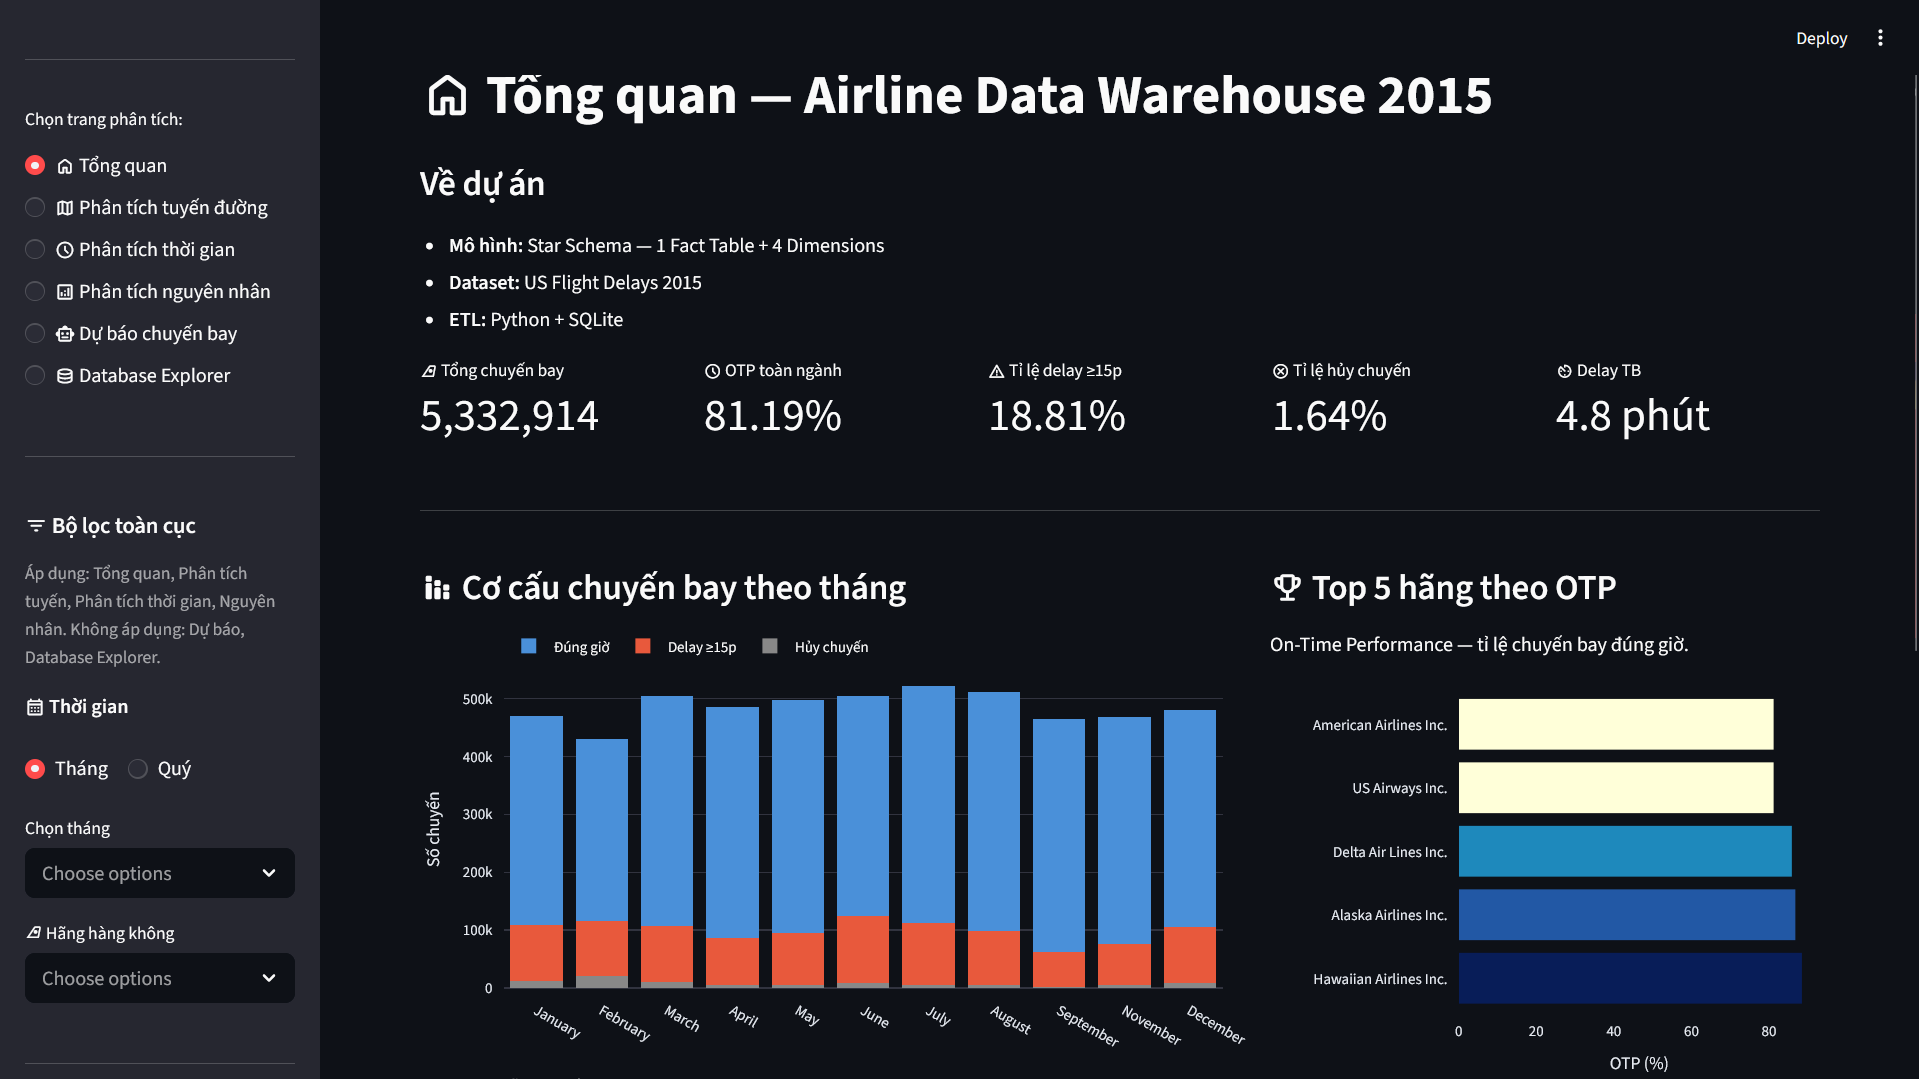
\includegraphics[width=\linewidth]{img/dashboard/overview.png}
    \caption{Trang Tổng quan: KPI, cơ cấu chuyến bay và xu hướng delay theo tháng.}
    \label{fig:dash_overview}
  \end{figure}

  \item \textbf{Phân tích tuyến đường:}
  Phân tích top tuyến bay (cặp sân bay đi $\to$ đến) theo từng hãng.
  Bộ lọc địa lý đặt ngay trên trang (không dùng sidebar): chọn \textbf{Bang xuất phát} / \textbf{Bang đích đến},
  sau đó lọc tiếp theo từng sân bay cụ thể.
  Hãng phân tích chọn ở sidebar; mỗi hãng được chọn sinh một khối biểu đồ riêng
  với số tuyến và ngưỡng số chuyến tối thiểu có thể điều chỉnh.
  \begin{figure}[H]
    \centering
    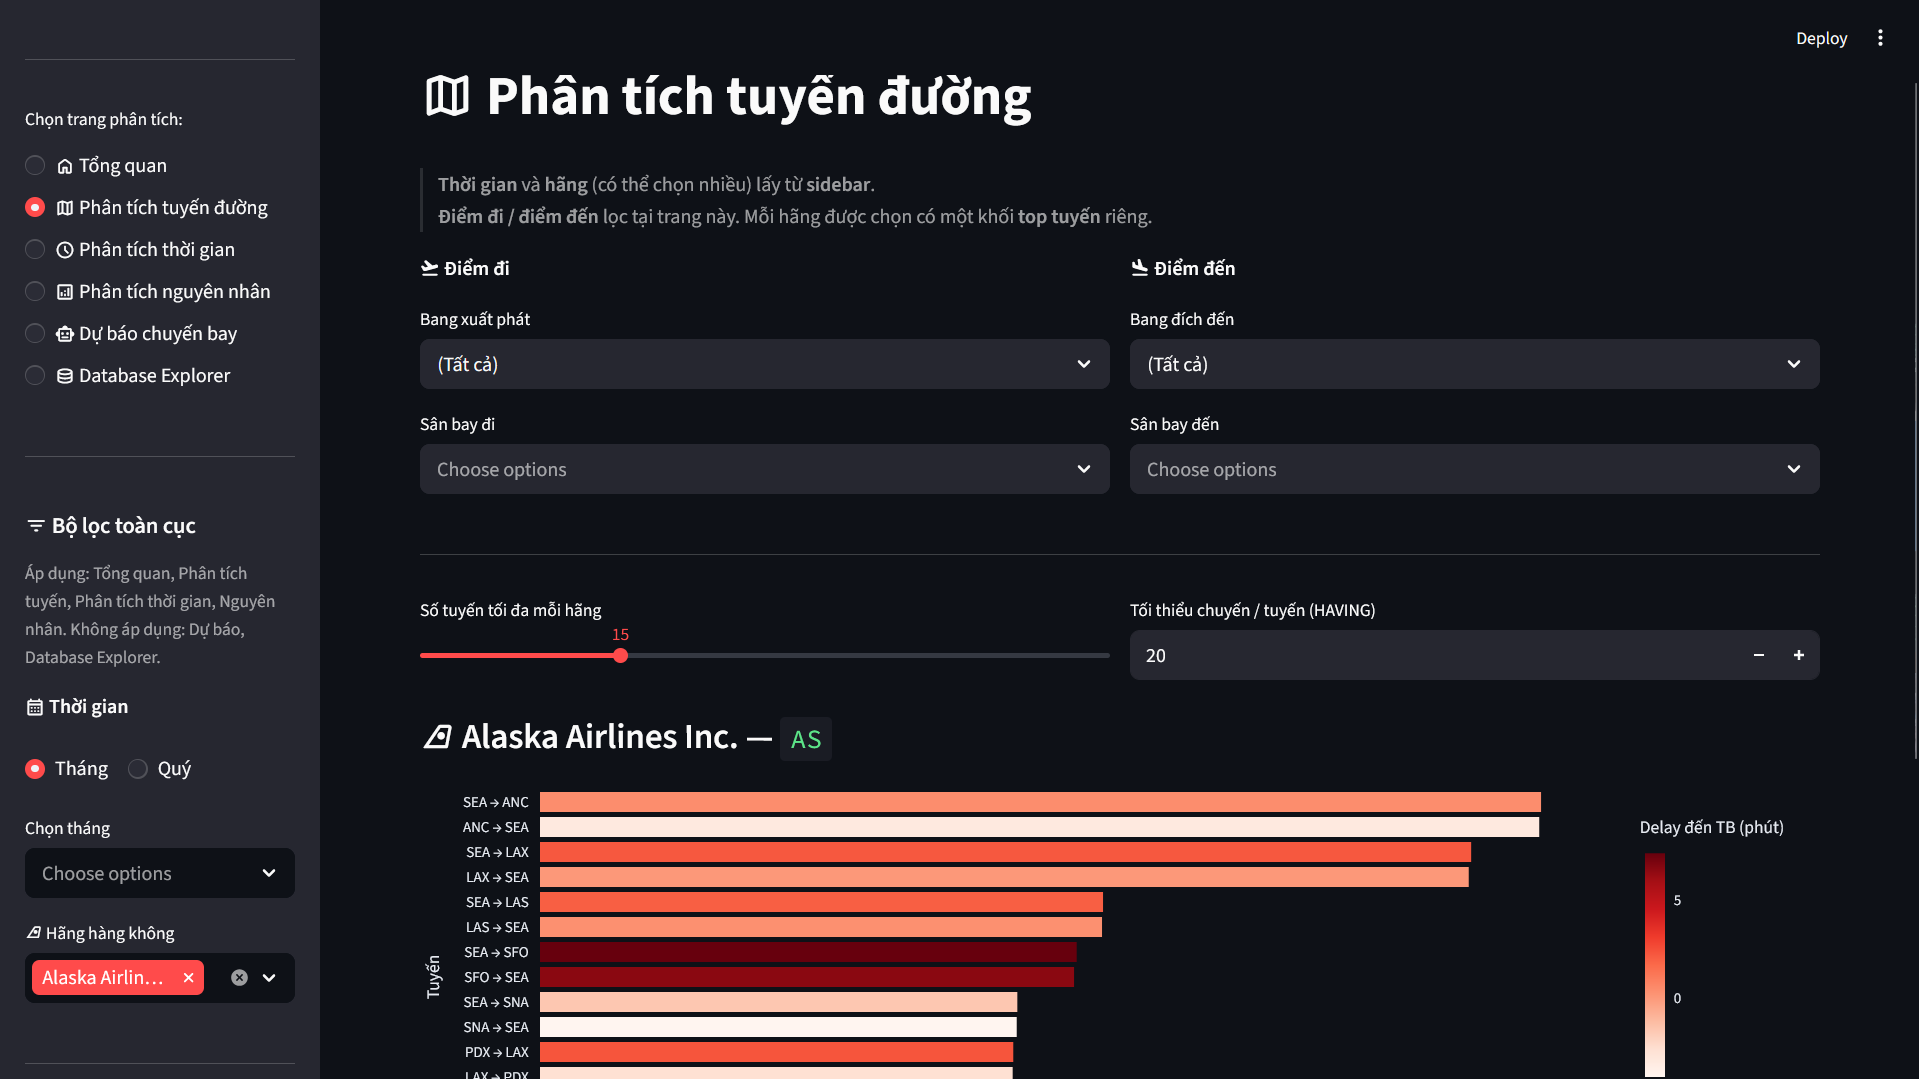
\includegraphics[width=\linewidth]{img/dashboard/routes.png}
    \caption{Trang Phân tích tuyến đường: lọc địa lý và top tuyến theo hãng.}
    \label{fig:dash_routes}
  \end{figure}

  \item \textbf{Phân tích thời gian:}
  Khám phá tính mùa vụ và chu kỳ của delay.
  Ở chế độ \textbf{Tháng}: heatmap phân bố số chuyến theo tháng $\times$ nguyên nhân;
  biểu đồ delay TB theo tháng tô màu theo mùa (xuân/hạ/thu/đông).
  Ở chế độ \textbf{Quý}: cột delay TB theo Q1--Q4.
  Ngoài ra luôn hiển thị: delay theo \textbf{thứ trong tuần} (hai panel: phút TB và tỷ lệ $\geq$15\%);
  so sánh nhanh \textbf{ngày thường} vs \textbf{cuối tuần} qua hai metric
  ($5{,}4$ phút so với $3{,}4$ phút khi không lọc);
  biểu đồ delay theo \textbf{4 khung giờ cất cánh} trong ngày.
  \begin{figure}[H]
    \centering
    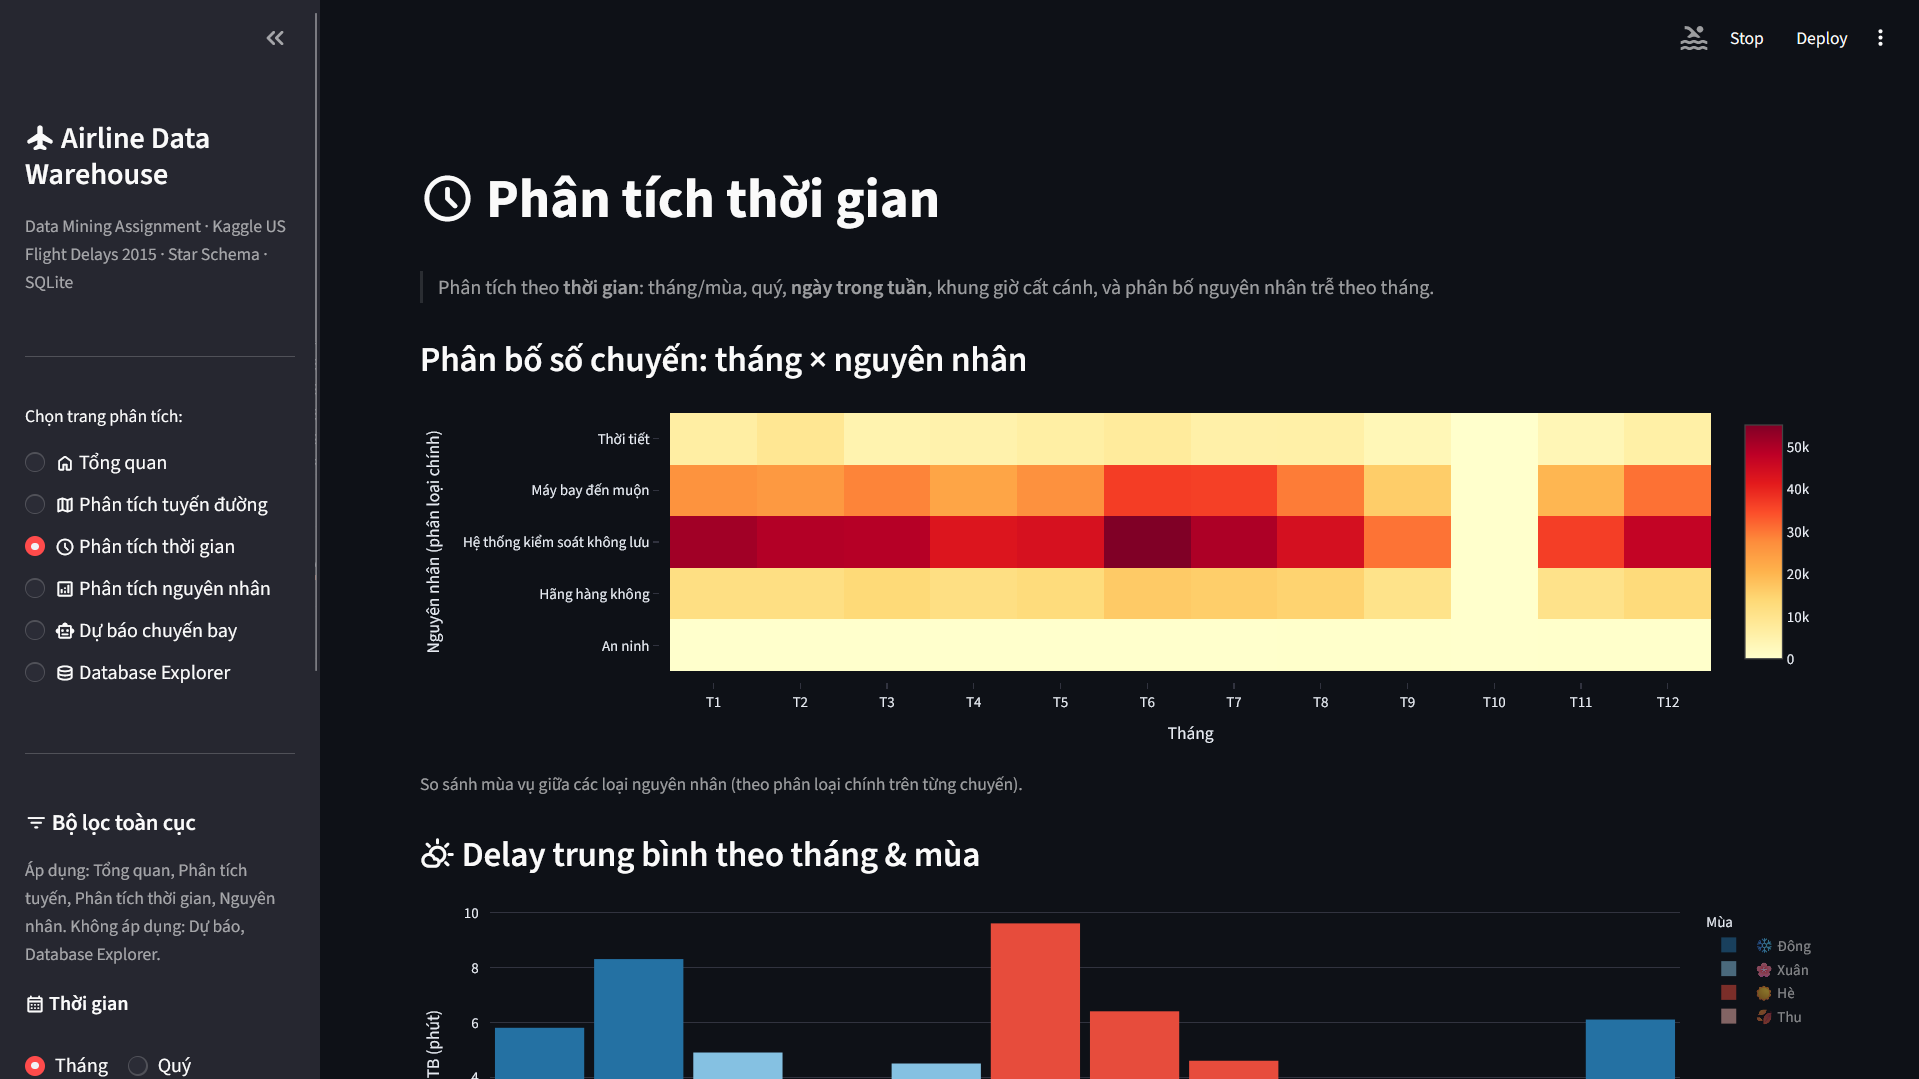
\includegraphics[width=\linewidth]{img/dashboard/time.png}
    \caption{Trang Phân tích thời gian: heatmap mùa vụ, thứ trong tuần và khung giờ bay.}
    \label{fig:dash_time}
  \end{figure}

  \item \textbf{Phân tích nguyên nhân:}
  Đi sâu vào cơ cấu gây trễ.
  Hai biểu đồ song song: pie cơ cấu số chuyến và cột ngang delay TB theo từng nguyên nhân
  (Hệ thống không lưu, Máy bay đến muộn, Hãng, Thời tiết, An ninh).
  Bảng tóm tắt đầy đủ với số chuyến, phần trăm, delay TB và tổng phút trễ theo từng loại.
  Cuối trang: biểu đồ \textbf{đóng góp tổng phút trễ} thể hiện nguyên nhân nào chiếm thời gian chờ lớn nhất.
  \begin{figure}[H]
    \centering
    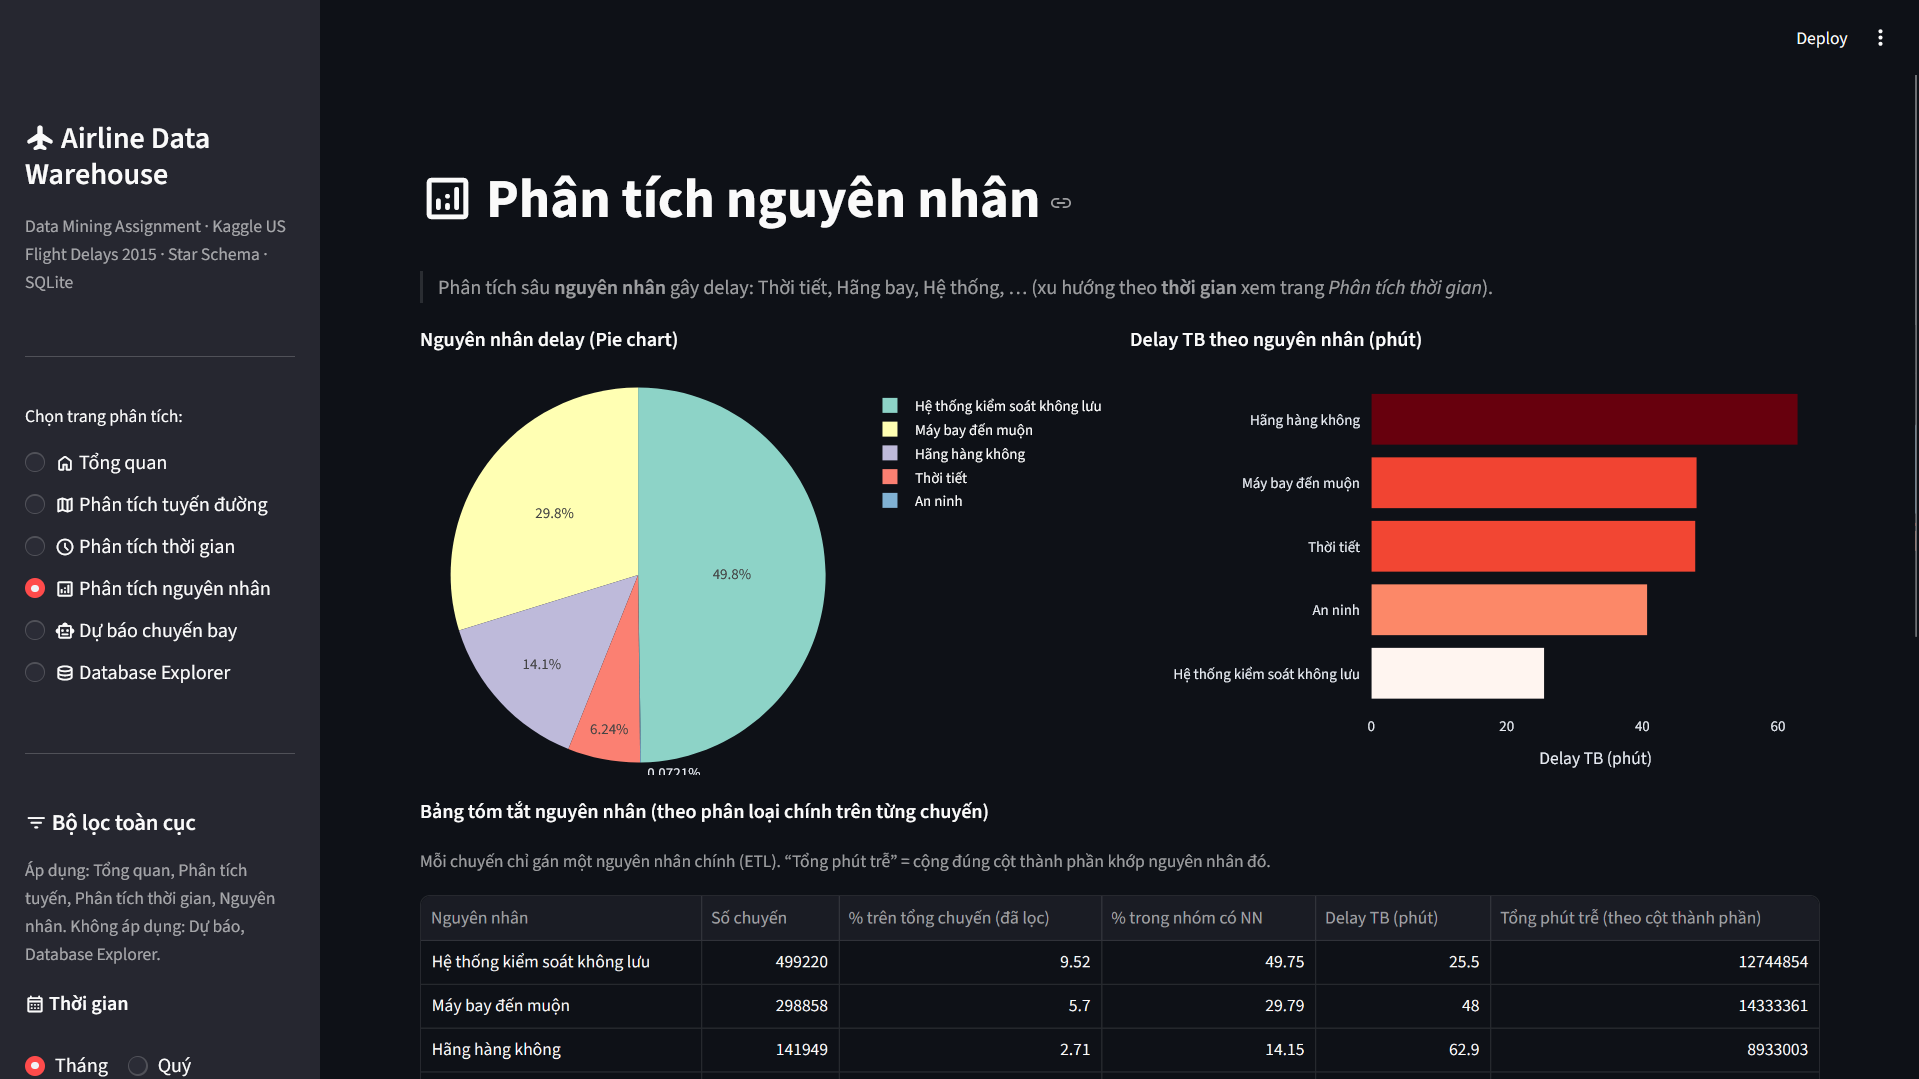
\includegraphics[width=\linewidth]{img/dashboard/reason.png}
    \caption{Trang Phân tích nguyên nhân: pie, delay TB và bảng tóm tắt theo loại nguyên nhân.}
    \label{fig:dash_reason}
  \end{figure}

  \item \textbf{Dự báo chuyến bay:}
  Cho phép người dùng nhập thông tin và nhận dự báo delay ngay trên giao diện.
  Form gồm: hãng, bang đi/đến, tháng, thứ trong tuần, giờ khởi hành (slider 0--23),
  khoảng cách và thời gian bay.
  Sau khi nhấn \textbf{Dự báo ngay}, hệ thống gọi \texttt{predict\_service}
  và trả về nhãn dự đoán (đúng giờ / có delay), xác suất delay và mức độ rủi ro,
  minh họa thêm bằng đồng hồ gauge Plotly.
  \begin{figure}[H]
    \centering
    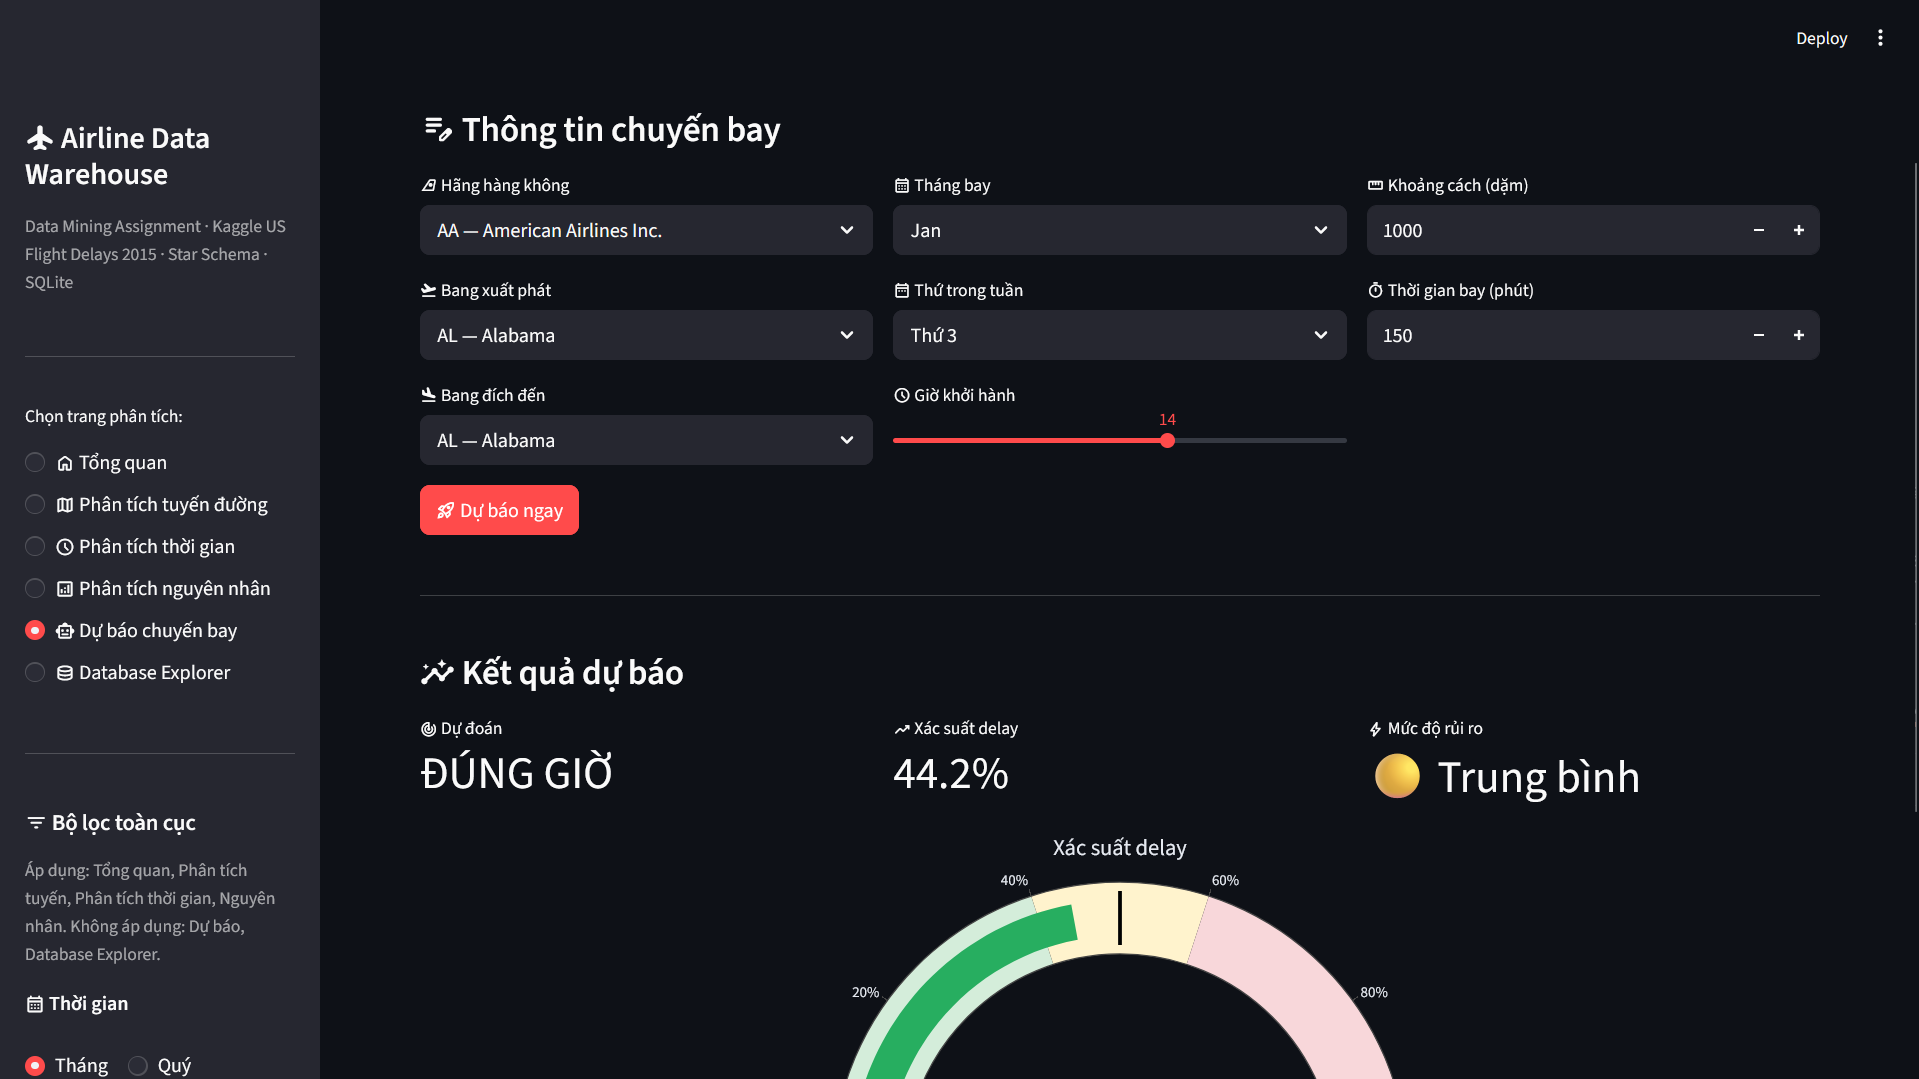
\includegraphics[width=\linewidth]{img/dashboard/predict.png}
    \caption{Trang Dự báo chuyến bay: form nhập liệu và kết quả dự báo với gauge xác suất.}
    \label{fig:dash_predict}
  \end{figure}

  \item \textbf{Database Explorer:}
  Công cụ tra cứu trực tiếp kho dữ liệu.
  Hiển thị sơ đồ Star Schema dạng ASCII và số dòng thực tế của từng bảng
  (\texttt{dim\_airline}: 14, \texttt{dim\_airport}: 322, \texttt{dim\_date}: 365,
  \texttt{dim\_delay\_reason}: 6, \texttt{fact\_flights}: $5\,332\,914$).
  Cho phép xem trước nội dung bất kỳ bảng nào với số dòng tùy chỉnh.
  Hỗ trợ nhập SQL tùy ý (chỉ \texttt{SELECT}); có nút Random/Clear/Execute và hiển thị kết quả tức thì.
  \begin{figure}[H]
    \centering
    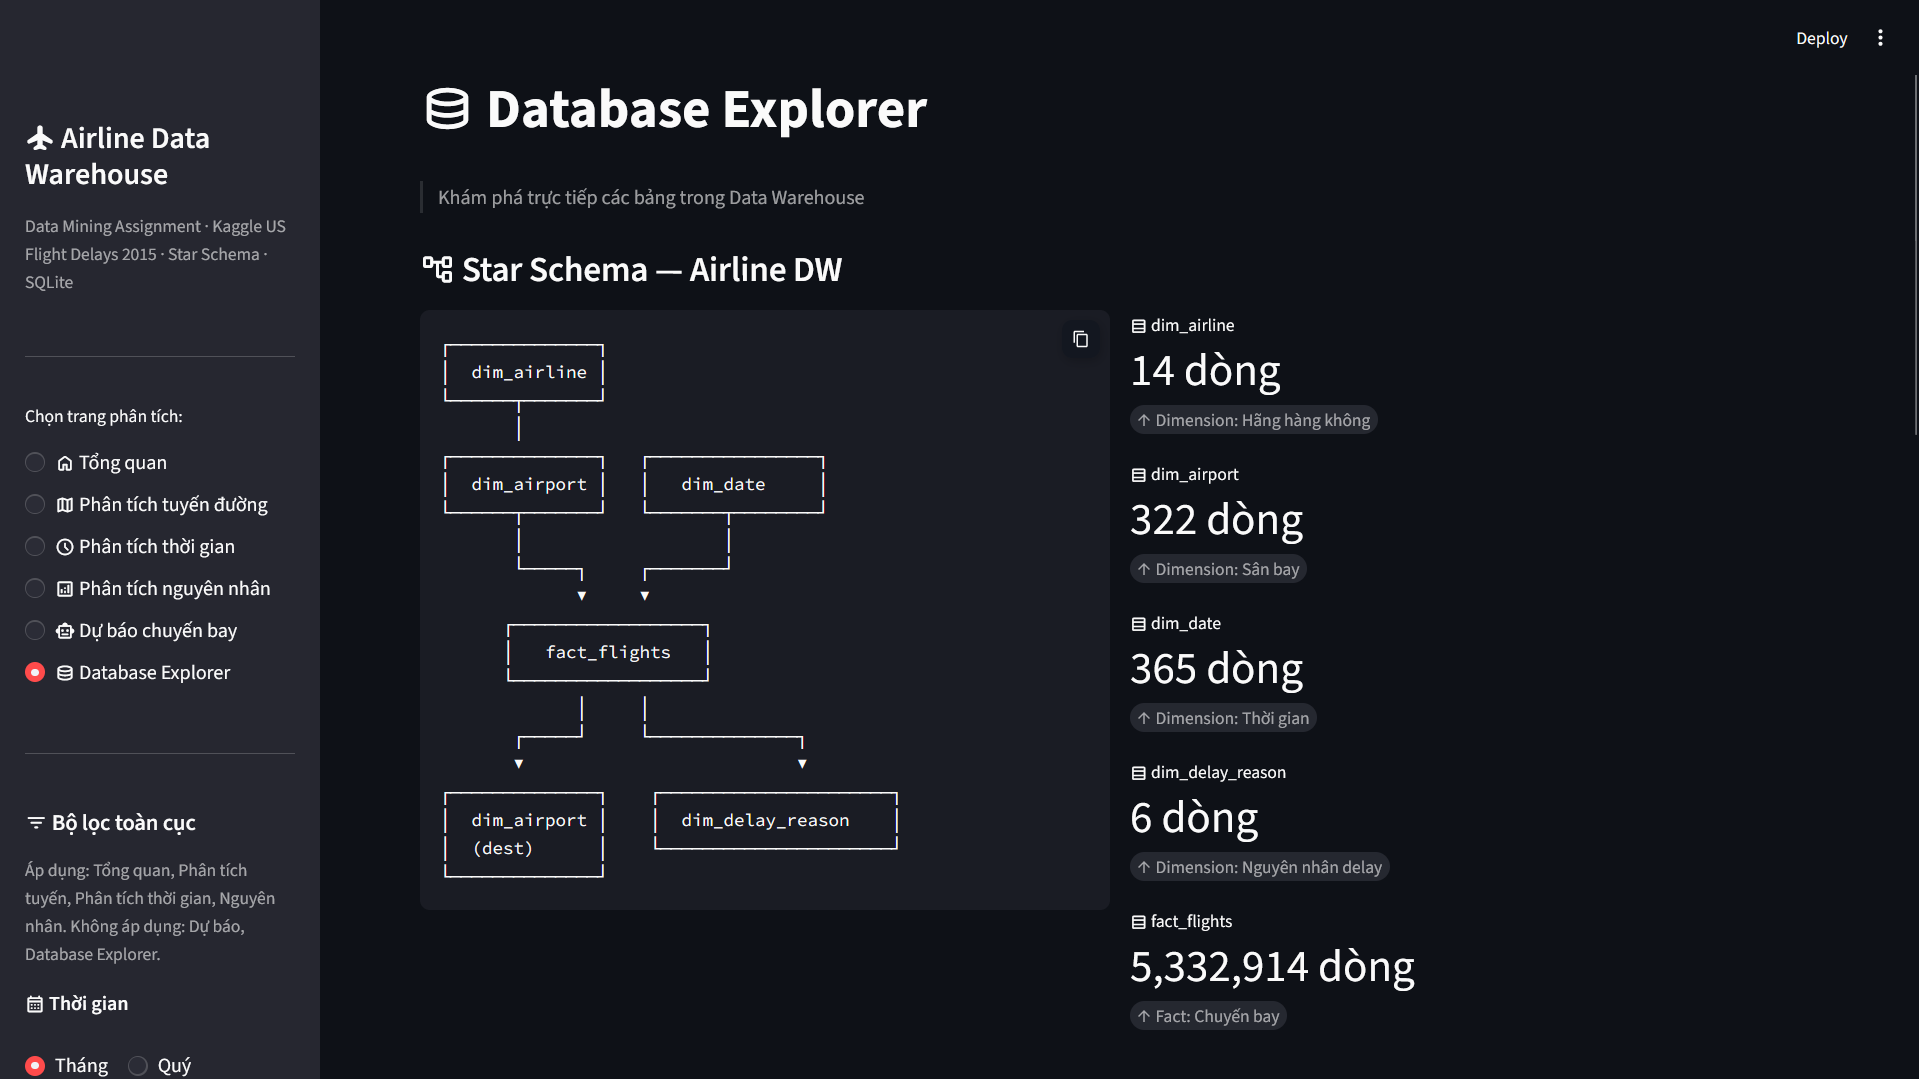
\includegraphics[width=\linewidth]{img/dashboard/database.png}
    \caption{Trang Database Explorer: sơ đồ star schema, thống kê bảng và SQL tùy chỉnh.}
    \label{fig:dash_explorer}
  \end{figure}

\end{enumerate}

\subsubsection{Mô hình khai phá: đặc trưng và tham số}

Nhãn: \texttt{is\_delayed\_15} (1 nếu \texttt{arrival\_delay} $\geq$ 15 phút).
Mô hình \textbf{không} sử dụng \texttt{departure\_delay} --- đây là quyết định có chủ đích:
departure delay chỉ biết \textit{sau khi} máy bay rời cổng, khiến mô hình mang tính
``phản ứng'' thay vì ``dự báo''. Thay vào đó, chỉ dùng các đặc trưng
biết trước hoặc có tính tổng hợp theo ngữ cảnh (bang, hãng, thời gian).

\begin{table}[H]
\centering
\caption{Mười đặc trưng đầu vào (hiện thực --- \texttt{compare\_5\_models.py})}
\small
\begin{tabular}{|l|l|l|}
\hline
\textbf{Đặc trưng} & \textbf{Kiểu} & \textbf{Lý do chọn} \\ \hline
\texttt{month}                & int   & Tính mùa vụ (bão hè, tuyết đông) \\ \hline
\texttt{day\_of\_week}        & int   & Thứ trong tuần (lưu lượng theo ngày) \\ \hline
\texttt{is\_weekend}          & int   & Cờ cuối tuần (T7 + CN) \\ \hline
\texttt{quarter}              & int   & Quý trong năm \\ \hline
\texttt{dep\_hour}            & int   & Giờ cất cánh (0--23, trích từ \texttt{scheduled\_departure}) \\ \hline
\texttt{distance}             & float & Quãng đường bay (dặm) \\ \hline
\texttt{elapsed\_time}        & float & Thời gian bay thực tế (phút) \\ \hline
\texttt{airline\_enc}         & int   & Mã hãng bay (Label Encoding từ \texttt{airline\_iata}) \\ \hline
\texttt{origin\_enc}          & int   & Bang sân bay đi (Label Encoding từ \texttt{state}) \\ \hline
\texttt{dest\_enc}            & int   & Bang sân bay đến (Label Encoding từ \texttt{state}) \\ \hline
\end{tabular}
\label{tab:features_impl}
\end{table}

Tham số huấn luyện tiêu biểu:
\begin{itemize}
  \item Logistic Regression: \texttt{saga} solver, C=1.0, \texttt{class\_weight='balanced'}, \texttt{max\_iter=200}.
  \item Random Forest: 100 cây, \texttt{max\_depth=10}, \texttt{min\_samples\_leaf=50}, \texttt{class\_weight='balanced'}.
  \item MLP (sklearn): [10$\to$64$\to$32$\to$1], ReLU, Adam adaptive, \texttt{alpha=0.001} (L2),
        \texttt{batch\_size=512}, early stopping (patience 5), tối đa 50 epoch.
  \item XGBoost: 300 cây, \texttt{max\_depth=6}, \texttt{lr=0.05}, \texttt{subsample=0.8},
        \texttt{scale\_pos\_weight} $\approx$ 3.76.
  \item LightGBM: 300 cây, \texttt{max\_depth=6}, \texttt{lr=0.05}, \texttt{subsample=0.8},
        \texttt{is\_unbalance=True}.
\end{itemize}

Mất cân bằng lớp ($\approx$81\% / 19\% trên chuyến \texttt{is\_cancelled=0} trong kho): dùng trọng số lớp thay vì over/undersampling vật lý;
đánh giá ưu tiên AUC-ROC và F1.
